\chapter{\label{chapter:preliminaries}Preliminaries and Methodology}

In this chapter, we will discuss all the necessary tools needed for this thesis. As we are considering asynchronous shared memory systems, the first section will cover the mathematical foundation for the computational model. This will include a formal description of concepts such as \emph{process},  \emph{algorithm}, and \emph{Linearizability~\cite{DBLP_journals_toplas_HerlihyW90}} in concurrent systems. In the following section, we delve into the hardware foundations of our concurrent systems. Specifically, we will explore concepts such as \emph{cache memory}, \emph{consistency memory model}, \emph{cache coherence}, and \emph{memory fences}, which are essential for implementing concurrent algorithms correctly. We will also discuss the concept of a memory model at the programming language level, and examine the Java and C++ memory models that define the allowable behavior of multithreaded programs. Finally, we will conclude this chapter by discussing the statistical experiment methodology we will use to analyze program implementations.

\section{\label{sec:computation-model}Computation Model}

We consider a standard concurrent shared memory system with \(n \ge 2\) \textit{asynchronous} processes, \(p_0, \ldots, p_{n-}\), which may \textit{crash} at any time during execution. The \textit{index} of process \(p_i\) is \(i\). Processes communicate with each other by invoking \textit{atomic} instructions of base objects: either simple \emph{Read}/\emph{Write}, or more powerful \emph{Read-Modify-Write}, such as \emph{Swap} or \emph{Compare\&Swap}.

An \emph{algorithm} for a high-level concurrent object \(T\) (e.g., a queue or a stack) is a distributed algorithm \(\mathcal{A}\) consisting of local state machines \(A_1,\ldots, A_n\). Local machine \(A_i\) specifies which instruction of base objects execute to return a response when it invokes a (high-level) operation of \(T\); each of these instructions is a \emph{step}.

An \emph{execution} of \(\mathcal{A}\) is a (possibly infinite) sequence of steps, namely, instructions of base objects, plus invocations and responses of (high-level) operations of the concurrent object \(T\) with the following properties:

\begin{enumerate}
    \item Each process first invokes an operation, and only when it has a corresponding response can it invoke another operation, i.e., executions are well-formed and
    \item For any invocation to an operation \(op\) of a process \(p_i\), denoted as \(inv_i(op)\), the steps of \(p_i\) between that invocation and its correspondent response (if there is one), denoted \(res_i(op)\), are the steps specified by \(A_i\) when \(p_i\) invokes \(op\).
\end{enumerate}

An operation in an execution is \emph{complete} if both its invocation and response appear in the execution. An operation is \emph{pending} if only its invocation appears in the execution. It is assumed that after a process completes an operation, it non-deterministically picks the operation it executes next. An execution \(E\) is an \emph{extension} of an execution \(F\), if \(E\) is a prefix of \(F\), namely, \(E = F\cdot F'\) for some \(F'\).

For any finite execution \(E\) and any process \(p_i\), \(E|p_i\) denotes the sequence of invocations and responses of \(p_i\) in \(E\). Two finite executions \(E\) and \(F\) are equivalent if \(E|p_i = F|p_i\) \(\forall p_i\). For any execution \(E\), \(comp(E)\) denotes the execution obtained by removing from \(E\) all steps and invocations of pending operations.

\hl{A process is \emph{correct} in an infinite execution if it takes infinitely many steps.} An implementation is lock-free if in every infinite execution, infinitely many operations are complete~\cite{DBLP_journals_toplas_HerlihyW90}. An implementation is \emph{wait-free} if, in every infinite execution, every correct process completes infinitely many operations~\cite {DBLP_journals_toplas_Herlihy91}. Thus, a wait-free implementation is lock-free but not necessarily vice-versa. \emph{Bounded wait-freedom}~\cite{DBLP_conf_spaa_Herlihy91} additionally requires that there is a bound on the number of steps needed to terminate. The \emph{step complexity} is the maximum number of steps a process needs to execute to return. The step complexity of an algorithm is the maximum among the step complexity of its operations.

In the \emph{Read-After-Write} synchronization pattern, a process first writes in a shared variable and then reads another shared variable, maybe executing other instructions in between. For example, this mechanism is widely used in the classic Lamport's bakery mutual exclusion algorithm (see for example,~\cite {DBLP_books_daglib_0020056}). The correctness of the mechanism requires that the write and read instructions of a process are executed in a specific order, although there is no data dependence relation between them.

An algorithm, or one of its operations, is \emph{fence-free} if it does not require any specific ordering among its steps beyond what is implied by data dependence (e.g. the value written by a \emph{Write} instruction depends on the value read by a previous \emph{Read} instruction). Note that a fence-free algorithm does not use \emph{Read-After-Write} synchronization patterns. In our algorithms, we use notation \(\{O_1.inst_1, \ldots, O_x.inst_x\}\) to denote that the instructions \(O_1.inst_1, \ldots, O_x.inst_x\) can be executed in any order. Observe that memory fences (also called memory barriers) are not required to correctly implement a fence-free algorithm in a concrete language or multi-core architecture since any reordering of non-data-dependent instructions does not affect the correctness of the algorithm.

\emph{Linearizability}~\cite{DBLP_journals_toplas_HerlihyW90} is the standard correctness condition for concurrent objects. Intuitively, an execution is linearizable if its (high-level) operations can be ordered sequentially, without reordering non-overlapping operations, so that their responses satisfy the specification of the implemented object.

A \emph{sequential specification} of a concurrent object \(T\) is a statute machine specified through a transition function \(\delta\). Given a state \(q\) and an invocation \(inv_i(op)\) of process \(p_i\), \(\delta(q, inv_i(op))\) returns the tuple \((q', res_i(op))\) (or a set of tuples if the machine is \emph{non-deterministic}) indicating that the machine moves to state \(q'\) and the response to \(op\) is \(res_i(op)\). The sequences of invocation-responses tuples \(\langle inv_i(op): res_i(op)\rangle\) produced by the state machine are its \emph{sequential executions}. For the sake of clarity, a tuple \(\langle inv_i(op): res_i(op)\rangle\) is simply denoted \(op\). Also, the subscripts of invocations and responses are omitted.

Given an execution \(E\), we write \(op <_E op'\) if and only if \(res(op)\) precedes \(inv(op')\) in \(E\). Two operations are \emph{concurrent} denoted \(op||_E op' \), if neither \(op <_e op'\) nor \(op' <_E op\). The execution is sequential \(<_E\) is a total order.

\begin{definition}[Linearizability~\cite{DBLP_journals_toplas_HerlihyW90}]
Let be \(\mathcal{A}\) an algorithm for a concurrent object \(T\). A finite execution \(E\) of \(\mathcal{A}\) is \emph{linearizable with respect to \(T\)}, or just \emph{linearizable} if \(T\) is clear from the context, if there is a sequential execution \(S\) of \(T\) and \(E\) can be extended to an execution \(E'\) by appending zero or more responses such that:

\begin{enumerate}
    \item \(comp(E')\) and \(S\) are equivalent and
    \item for every two complete operations \(op\) and \(op'\) in \(E\), if \(op <_E op'\) then \(op <_S op'\).
\end{enumerate}

We say that \(\mathcal{A}\) \emph{is linearizable with respect to} \(T\) or just \emph{linearizable} if \(T\) is clear from the context if each of its executions is linearizable.
\end{definition}

Roughly speaking, while linearizability requires a total order of the operations, \emph{set-linearizability}~\cite{DBLP_journals_jacm_CastanedaRR18, DBLP_conf_podc_Neiger94} is an extension of linearizability that allows several operations to be linearized at the same linearization point.

A \emph{set-sequential specification} of a concurrent object differs from a sequential execution in that \(\delta\) receives as input the current state \(q\) of the machine and set \(Inv = \{inv_{id_1}(op_1), \ldots, inv_{id_t}(op_t)\}\) of operation invocations, and \(\delta(q, Inv)\) returns \((q', Res)\), where \(q'\) is the next state and \(Res = \{res_{id_1}(op_1), \ldots, res_{id_t}(op_t)\}\) are the responses to the invocations in \(Inv\) and each \(id_i\) denotes the index of the invoking/responding process. Intuitively , all operations \(op_1, \ldots, op_t\) are performed concurrently and move the machine from state \(q\) to \(q'\). The sequence of sets \(Inv\), \(Res\) is a \emph{concurrency class} of the machine. The state machine's sequences of concurrency classes are its \emph{set-sequential executions}. In our set-sequential specifications, invocations will be subscripted with the index of the invoking process only when there is more than one invocation in a concurrency class. Observe that a set-sequential specification in which all concurrency classes have a single element corresponds to a sequential specification.

Give a set-sequential execution S of a set-sequential object, the partial order \(<_S\) on the operations of \(S\) is defined as above: \(op <_S op'\) if and only if \(res(op)\) precedes \(inv(op')\) in \(S\), namely, the concurrency class of \(op\) appears before of the concurrency class of \(op'\).


\begin{definition}[Set-linearizability~\cite{DBLP_journals_jacm_CastanedaRR18, DBLP_conf_podc_Neiger94}]
    Let be \(\mathcal{A}\) an implementation of a concurrent object \(T\). A finite execution \(E\) of \(\mathcal{A}\) is \emph{set-linearizable with respect to} \(T\), or just \emph{set-linearizable} if \(T\) is clear from the context, if there is a set-sequential execution \(S\) of \(T\) and \(E\) can be extended to an execution \(E'\) by appending zero or more responses such that:

    \begin{enumerate}
        \item \(comp(E')\) and \(S\) are equivalent,
        \item for every two completed operations \(op\) and \(op'\) in \(E\), if \(op <_E op'\) then \(op <_S op'\).
    \end{enumerate}

    We say that \(\mathcal{A}\) is \emph{set-linearizable with respect to} \(T\), or just \emph{set-linearizable} if \(T\) is clear from the context if each of its executions is set-linearizable.
\end{definition}

\section{\label{sec:hardware-foundations}Hardware Foundations}

In addition to the mathematical computation model, understanding the hardware foundations behind concurrent computing is important. Understanding this helps to explain why certain tools, such as ``\emph{fences}'' are necessary to ensure correct concurrent computing. This section will discuss the high-level working of concurrent programs on computer hardware. Our focus will be on memory interactions at different levels. 

When analyzing computer systems, it is important to consider those with multi-core processors that share memory. This means all cores can perform loads and stores to all (physical) addresses. A typical system model includes a single chip with multiple cores and off-chip main memory. You can see an illustration of this in the figure~\ref{fig:multi-core-processor}\footnote{In the figure~\ref{fig:multi-core-processor}, we omit many features to simplify the reasoning about the hardware}. Usually, a multi-core processor includes \emph{cache memory}, a special high-speed memory close to the processor that allows fast process access. Caches decrease the average latency when accessing storage structures~\cite{DBLP_series_synthesis_2020Nagarajan}. Multi-core chips in recent times have adopted a three-tiered cache memory system. The first two levels, L1 and L2, are private to each core, while the third level, L3, is shared by all the cores. The main objective of L1 and L2 is to enable fast access to data and instructions for the core. Each core utilizes the first cache level in a computer system to fetch the required data and execute instructions. Cache L1 is split into two sub-caches, one for data (L1d) and the other one for instructions (L1d) that will fetched by the core. Typically, the access to this level of cache is faster than that of other levels. The second level of cache is generally larger and stores data and instructions about to be executed. Multiple cores share the third cache level and serve as a source for the L2 cache.

The \emph{main memory} holds frequently accessed data for the CPU, such as instructions or processing data, and allows faster access than secondary memory. To obtain such data and instructions, the processor calls the \emph{memory bus}, which transfers data from the primary memory to the CPU and cache memory. This bus has two parts: the data bus and the address bus. The data bus transfers information between the primary memory and the corresponding chipset. On the other hand, the address bus is used to retrieve information about the location of stored data.

When considering the simplified view of cache architecture, it is important to ensure that shared memory is correct. This requires addressing two key issues: \emph{consistency} and \emph{correctness}.
The consistency provides rules about loads and stores (memory reads and writes) and how they act upon memory. These consistency rules must consider the behavior of those operations on memory through access to multiple threads or even a single thread. The consistency models define correct shared memory behavior regarding loads and stores without reference to caches or coherence \cite{DBLP_series_synthesis_2020Nagarajan}. Shared memory correctness is specified by a memory consistency model (or memory model). This defines the allowed behavior of multithreaded programs executing with shared memory. The most intuitive and strongest memory model is the \emph{Sequential Consistency} (SC) [referencia]. Another memory model used by systems \emph{x86} and \emph{SPARC} is \emph{Total Store Order} (TSO) [referencia], motivated by the desire to use \emph{first-in-first-out} write buffers to hold the results of committed stores before writing results to the caches. In addition to the prior memory model, "relaxed" or "weak" memory models are considered because these models show that most memory orderings in strong models are unnecessary \cite{DBLP_series_synthesis_2020Nagarajan}.

\begin{figure}
    \centering
    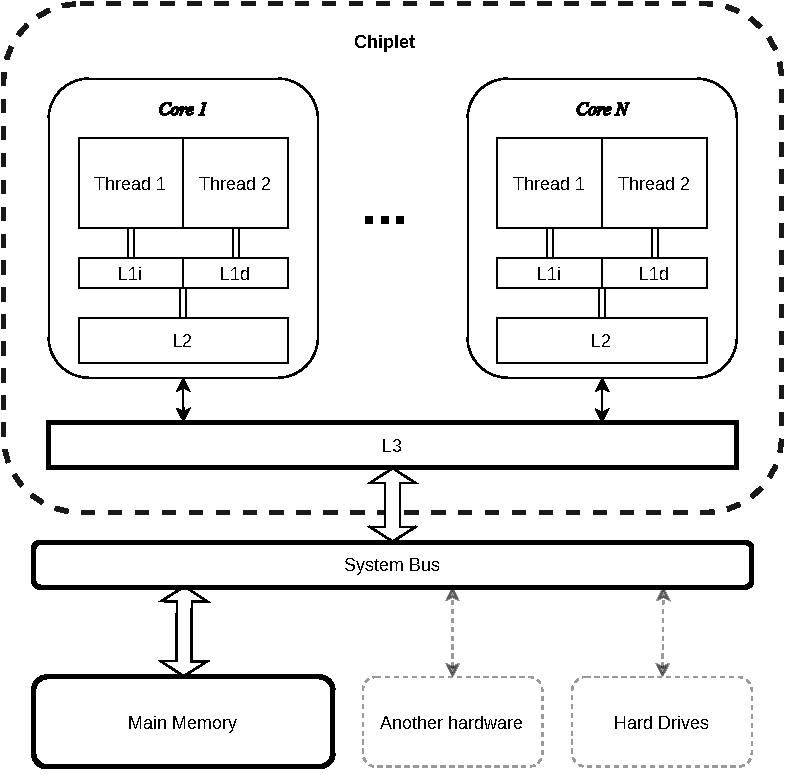
\includegraphics[width=0.7\linewidth]{contents//figures/III_2_cpu.pdf}
    \caption{Baseline model of a Multicore Processor Chip}
    \label{fig:multi-core-processor}
\end{figure}

Cache coherence protocols play an important role in solving coherence issues in caching. These protocols come into play when multiple cores have access to multiple copies of a datum, each in a core, and at least one is a write access. To prevent access to stale or incoherent data, a set of rules is implemented by the distributed set of cores within a system. Therefore, along with consistency models, it is essential to consider cache coherence protocols. These protocols use the common MOESI coherence states: modified (M), owned (O), exclusive (E), shared (S), and invalid (I). The protocol acts like a state machine, moving from one state to another based on the conditions of the data and the cache memory \cite{DBLP_series_synthesis_2020Nagarajan}.

A memory fence is a barrier instruction that causes a CPU or compiler to enforce an ordering constraint on memory operations (loads and stores) issued before and after the barrier instruction. These instructions are necessary because most modern CPUs or compilers employ performance optimizations, changing the order of the instructions on one program, which could result in out-of-order execution. Typically, these optimizations are unnoticed in a single-thread program but can cause unpredictable behavior in concurrent programs. For example, consider the following multi-thread program with two threads, each one concurrently running in distinct cores, the first one executing the code shown in~\ref{lst:thread1}, and the second one executing the code shown in~\ref{lst:thread2}:

\begin{lstlisting}[language=c++,label={lst:thread1}, caption={Thread 1, core 1} ,captionpos=b]
while (z == 0);
print(y);
\end{lstlisting}

\begin{lstlisting}[language=c++,label={lst:thread2} ,caption={Thread 2, core 2} ,captionpos=b]
y = 30;
z = 1;
\end{lstlisting}

In this case, we might expect that the \texttt{print(y)} always prints the number 30. Nevertheless, the compiler or the CPU could change the order of the instructions for thread 2, giving as a result, an execution where the value for \texttt{y} is undefined, and the instructions could be interleaved as shown in the code~\ref{lst:reordering}:

\begin{lstlisting}[language=c++,label={lst:reordering},caption={Code reordered by CPU} ,captionpos=b]
z = 1; // Thread 2
while (z == 0); // Thread 1
print(y); // Thread 1
y = 30; // Thread 2
\end{lstlisting}

This execution is sequentially consistent but is an out-of-order execution producing an undefined result. With the use of memory barriers, we can ensure that instructions do not be reordered. For example, our code could be rewritten as follows:

Thread 1, core 1.
\begin{lstlisting}[language=c++,label= ,caption= ,captionpos=b,numbers=none]
while (z == 0);
fence()
print(y);
\end{lstlisting}

Thread 2, core 2.
\begin{lstlisting}[language=c++,label= ,caption= ,captionpos=b,numbers=none]
y = 30;
fence();
z = 1;
\end{lstlisting}


Languages such as \texttt{Java} or \texttt{C++} provide instructions to establish synchronization
and ordering constraints between threads without an atomic operation. These
instructions have semantics well-defined for

In the case of Java, we have static methods of the class VarHandle\footnote{\texttt{java.lang.invoke.VarHandle}}. Those are memory fence methods that help provide fine-grained control of memory ordering. These statics
methods are \cite{varHandleJdk92017}:

\begin{description}
\item[{fullFence}] Ensures that loads and stores before the fence will not be
reordered with loads and stores after the fence. This method has memory
ordering effects compatible with
\texttt{atomic\_thread\_fence(memory\_order\_seq\_cst)}.
\item[{acquireFence}] Ensures that loads before the fence will not be reordered
with loads and stores after the fence. This method has memory ordering
effects compatible with \texttt{atomic\_thread\_fence(memory\_order\_acquire)}.
\item[{releaseFence}] Ensures that loads and stores before the fence will not
be reordered with stores after the fence. This method has memory ordering
effects compatible with \texttt{atomic\_thread\_fence(memory\_order\_release)}.
\item[{loadLoadFence}] Ensures that loads before the fence will not be
reordered with loads after the fence.
\item[{storeStoreFence}] Ensures that stores before the fence will not be
reordered with stores after the fence.
\end{description}

For C++, we have the function
\texttt{std::atomic\_thread\_fence}\cite{threadFenceCpp2020}, which establishes
memory synchronization ordering of non-atomic and relaxed atomic access, as
instructed by order, without an associated atomic operation. The type of
synchronization that can handle the following:

\begin{itemize}
\item Fence-atomic synchronization
\item Atomic-fence synchronization
\item Fence-Fence Synchronization
\end{itemize}

Using a memory order\cite{memoryOrderCpp2020}, it can specify how memory accesses, including regular, non-atomic memory accesses, will be
ordered around an atomic operation. There are six orders, from the
relaxed memory order to the sequentially consistent memory order. They are:
\texttt{memory\_order\_relaxed}, \texttt{memory\_order\_consume}, \texttt{memory\_order\_acquire},
\texttt{memory\_order\_acq\_rel} and \texttt{memory\_order\_seq\_cst}. A note about
\texttt{atomic\_thread\_fence} functions is that on x86 (x86\textsubscript{64}), these functions
issue no CPU instructions and only affect compile time code, with the exception
for \texttt{std::atomic\_thread\_fence(std::memory\_order::seq\_cst)}, which issue the
full memory fence instruction \texttt{MFENCE}.

\subsection{Memory management}
\label{sec:org1ca9ee9}

To implement efficiently the idempotent algorithms in an environment without
garbage collection, it's necessary to use some technique or methodology to
provide garbage collection when atomic pointers are used or when distinct
threads want to reclaim the memory of the object associated with the pointer.

\begin{enumerate}
\item Strategies to delete shared pointers
\label{sec:org36ce5a6}

\begin{itemize}
\item Add pointers to list to safety delete.
\item Do this when there aren't more threads accessing methods.
\begin{itemize}
\item Increase the counter when a thread enters the method and decrease when
it exits.
\item Delete all pointers when the counter is equal to zero.
\end{itemize}
\end{itemize}


\item Hazard pointers
\label{sec:org3992578}

The \emph{Hazard Pointers} is a technique to manage language memory without garbage collectors. Maged proposed this technique
Michael \cite{DBLP_journals_tpds_Michael04}. They are so-called because
deleting a pointer that might be referenced by other thread(s) is
dangerous. If another thread keeps holding references to that pointer and
proceeds to access that pointer after being deleted, you have an undefined
behavior \cite{DBLP_journals_tpds_Michael04}.

The basic idea of this technique is the following:

\begin{itemize}
\item If a thread wants to use a pointer that another thread might want to
delete, it first sets a hazard pointer to the pointer, informing the
other thread that deleting it would be dangerous. Once the object
is no longer needed, the hazard pointer is cleared.
\item When a thread wants to delete the pointer, it must check if the hazard
pointers belong to the other threads in the system. If no one has a
reference to the pointer, then it's safe to delete it. Otherwise, it must be left until later.
\item Periodically, we must check the list of objects that have been left until
later to see if any of them can be deleted now.
\end{itemize}

A general pseudocode for this technique could be the following:

\begin{lstlisting}[language=c++,label= ,caption= ,captionpos=b,numbers=none]
void func() {
    std::atomic<void*>& hp = get_hazard_pointer_for_current_thread();
    void* old_data = data.load();
    do {
        void* temp;
        do{ // Loop until you've set the hazard pointer
            temp = old_data;
            hp.store(old_data);
            old_data = data.load();
        } while (old_data != temp);
          }while (old_data &&
            !data.compare_exchange_strong(old_data, old_data->next);
    // Do something with old_data
    hp.store(nullptr); // clearing usage of hazard pointer
    // Trying clearing
    if (outstanding_hazard_pointers_for(old_head))
    {
        reclaim_later(old_data);
    }
    else
    {
        delete old_data;
    }
    delete_nodes_with_no_hazards();
}
\end{lstlisting}


\item Atomic Smart Pointers (Herlihy, Chapter 19) (Not available for GCC and CLang)
\label{sec:org58c7cdb}


When a memory region is reclaimed, the programmer cannot know how that
region of memory will be reused or whether it is reused. We need a
way of developing a (general) solution to prevent the sorts of races
when a memory region is reclaimed by many threads asynchronously. We can
do this by delaying reclamation.
Thinking in terms of pending operations on a concurrent data structure, a
sufficient condition is that \emph{memory is only reclaimed when it is impossible
for any pending operation to access in the future}.

This property could also be achieved by \emph{reference counting}. In a reference
counted implementation of a data structure (like a list), a counter of type
atomic<int> is associated with each node. Whenever a reference to node N is
created
\end{enumerate}

\section{\label{sec:practical-model}Language Model of Computation}
\section{\label{sec:methodology}Experimental Methodology}

\label{sec:orgebd0619}

To evaluate the performance of our Queue, we design a set of experiments that
allow us to know if the Queue is competitive against other queues in the
literature. We divide our experiments into two classes: \emph{inner experiments}
\sout{(this name could change in the future)} and \emph{outer experiments}. We used the
inner experiments to know which one of our implementations (LL/IC object and
Queue based on distinct variants of the LL/IC objects) have the best
performance and throughput. Once the inner experiments and the best
option are chosen, we evaluate the Queue against queues in state of the
art. We compare our Queue against:

\begin{enumerate}
\item Queue from Michael and Scott \cite{DBLP_conf_podc_MichaelS96}.
\item Queue from Yang and Mellor-Crummey \cite{DBLP_conf_ppopp_YangM16}.
\item We try to compare against the Queue from Ostrovsky and Morrison, but we
are limited by hardware \cite{scalingconcurrent2020}. (Possible change).
\end{enumerate}

We follow and adapt the guidelines shown in
\cite{lilja2005measuring, DBLP_conf_oopsla_GeorgesBE07, forsyth2018probability} to perform such evaluation. In
these guidelines, they explain how to measure computer performance using
fundamental techniques to analyze and understand the performance of computer
systems. They also discuss performance metrics, strategies used in
benchmark programs, and statistical tools to interpret measured performance
data.

\subsection{Inner Experiments}
\label{sec:org4649774}

To evaluate the performance of our distinct variants for the LL/IC Object
and the Queue, we perform the following experiments:

\begin{enumerate}
\item For an initial empty LL/IC Object, we perform a fixed number of calls to
LL/IC pairs. In each iteration, a thread executes a call to the LL method
followed by a call to the IC method. These calls are spread evenly among
a fixed number of threads, which work concurrently. Each thread performs
a random amount of "fake work" between both calls to avoid long-run
scenarios
\cite{DBLP_conf_ppopp_YangM16,DBLP_conf_podc_MichaelS96}. This fake
work is just an empty spin.
\item To test our concurrent Queue, we perform two benchmarks. The first one is
to perform enqueue-dequeue pairs similar to the previous experiment. In
the second one, in each iteration, each thread decides randomly to
execute a dequeue or enqueue with the same probability. The total of
calls is partitioned evenly among all threads.
\end{enumerate}


\subsection{Update experiments}
\label{sec:org5027fac}

To update the experiments, we must understand what metrics
allow us to compare the algorithms designed for LL/IC objects and Baskets. A
common way to evaluate experimental results is the use of measurements to
understand the performance or the throughput of the experiments;
but what is the meaning of performance and throughput? According to the
Cambridge Dictionary, \emph{Throughput} is the amount of work done in a particular
period; on the other side, performance is how well someone or something
functions, works, etc. Conversely, \emph{Performance} refers to the amount
of useful work a system accomplices. Performance usually is measured in
terms of accuracy, efficiency, and speed of executing instructions. From
\cite{lilja2005measuring}, some strategies for measurement are:

\begin{description}
\item[{Event driven}] It records the information necessary to calculate the
performance metric whenever an event occurs.
\item[{Tracing}] Similarly to the previous, but instead of recording the event
that has occurred, a portion of the system is recorded to identify the event.
\item[{Sampling}] This strategy records a portion of the system in a fixed time
interval.
\item[{Indirect measurement}] This type occurs when the metric data is not
directly accessible, and you must find another metric that can be measured
directly.
\end{description}

We can combine those strategies with the use of interval timers to measure
how much time it takes to execute the program or some section of code; this can
also provide a time basis for sampling.

In \href{https://en.wikipedia.org/wiki/Computer\_performance}{terms of computing}, the performance refers to the amount of useful
work accomplished by a computer system. Computer performance is measured in
terms of accuracy, efficiency, and speed of executing computer program
instructions. One or more of the following factors might be involved:

\begin{enumerate}
\item Short response time for a given piece of work.
\item High throughput.
\item Low utilization of computing resources.
\item High availability of a computing system.
\item High bandwidth.
\item Short data transmission time.
\end{enumerate}

To begin with a performance-analysis problem, three techniques can be used to find the desired solution:

\begin{enumerate}
\item Measurements of existing systems.
\item Simulation.
\item Analytical modeling.2
\end{enumerate}

Some benchmarks used to test concurrent queues are:

\begin{itemize}
\item enqueue - dequeue pairs:
\item 50\% enqueues
\end{itemize}

In both benchmarks, some work is added to avoid long-run scenarios. This
anomaly is described in \cite{DBLP_conf_podc_MichaelS96} and to avoid it, the
work added consists of spinning a small amount of time (6 \(\mu\)s) in an
empty loop. The idea behind this is to prevent long runs of queue operations
by the same process without this being interrupted, so this would display
an overly optimistic performance due to the lower cache miss rate.


\subsection{Statistics tools for experiments}
\label{sec:orga1c9a7a}

To evaluate our modular queue with all its variants, we need to determine a
methodology to know their performance and the throughput of each
variant. Also, we need to compare them with other queue algorithms in the
literature to check if it is competitive. We will divide the experiments into
two categories; the first is related to measuring the performance of the
distinct variants described previously. The second is to compare our best
queue algorithm (or the two best) to related queue algorithms in the
literature. To know the performance of our algorithms, we want to measure the
time required to execute a set of operations over an interval of time, i.e.,
how quickly complete its execution the program. The technique used to measure
the time of an event is the following:

\begin{itemize}
\item Read the current time and store it in a variable \texttt{start\_count}.
\item Let the portion of the program execute.
\item Read the current time and store it in a variable \texttt{stop\_count}.
\item Take the difference between \texttt{start\_count} and \texttt{stop\_count}. This will be the
total time required to execute the event.
\end{itemize}

This technique for measuring the execution time of any portion of a program
is known as the \emph{wall clock} time\cite{lilja2005measuring}. All the events we
want to measure will use this technique to get their execution time.
However, this measurement includes the time spent on other system operations,
like memory paging, thread interleaving, input/output operations, and network
communication, if applicable. Those external events could introduce
uncertainty into our measurements. We refer to these uncertainties in
measurements as errors or noise. To know how much uncertainty exists, we must
use probability and statistics tools to quantify it. To summarize a
collection of measures, we can use indices of central tendency (the mean, the
median, and the mode). The most commonly used index is the (sample
arithmetic) mean or average, which can summarize all the measurements
performed into a single number that somehow represents the center of the
distribution of these values. To quantify the precision of our measurements,
we can use a \emph{confidence interval} for the mean
value\cite{lilja2005measuring, DBLP_conf_oopsla_GeorgesBE07}. Other tools we
need are the \emph{sample variance}, the \emph{standard deviation}, and the \emph{coefficient of
variation}. Formally, the \emph{(sample arithmetic) mean} is defined to be:

\begin{equation}
\bar{x}_A = \frac{1}{n}\sum^n_{i = 1}x_i
\end{equation}

Where \(x_i\) values the individual measurements. The \emph{sample variance}
represent our calculated estimate of the actual variance. It is defined to be:

\begin{equation}
s^2 = \frac{\sum_{i = 1}^n(x_i - \bar{x}^2)}{n - 1}
\end{equation}

Where the \(x_i\) are the \(n\) independent measurements and \(\bar{x}\) is
the corresponding sample mean. From the previous equation, the standard
deviation is defined as the positive square root of the variance:

\begin{equation}
s = \sqrt{s^2} = \sqrt{\frac{\sum_{i = 1}^n(x_i - \bar{x}^2)}{n - 1}}
\end{equation}

The coefficient of variation (COV) is defined to be:

\begin{equation}
  COV = \frac{s}{\bar{x}}
\end{equation}

Suppose we can approximate the distribution of random errors by a Gaussian
distribution. In that case, we determine how well our estimate of the true value is concerning the actual true value using the properties of the distribution. We use
confidence intervals to find a range of values with a probability
of including the true value. To do that, we must consider two cases:

\begin{enumerate}
\item When the number of measurements is large \((n \ge 30)\).
\item When the number of measurements is small \((n < 30)\).
\end{enumerate}

For the first case, we use the sample mean \((\bar{x})\) as the best
approximation of the true value. If the \(n\) samples used to calculate
\(\bar{x}\) are all independents with mean \(\mu\) y standard deviation
\(s\), the central limit theorem then assures us that, for large values of
\(n\), the sample mean \(\bar{x}\) is approximately Gaussian distributed with
mean \(\mu\) and standard deviation \(s / \sqrt{n}\). We can quantify the
precision of the measurements searching two values \(c_1\) and \(c_2\), such
that the probability of the mean value being between those two values is \(1 -
   \alpha\). That is \(PR[c_1 \le \bar{x} \le c_2] = 1 - \alpha\). \(c_1\) and
\(c_2\) are chosen to form a symmetric interval around \(\bar{x}\) such that
\(Pr[x < c_1] = Pr[x > c_2] = \frac{\alpha}{2}\). The interval \([c_1, c_2]\)
is called \textit{confidence interval} for \(\bar{x}\) and \(\alpha\) is
called the \textit{significance level} and the value \((1 - \alpha)\) is
called the \textit{confidence level}. From the central limit theorem, we
have:

\begin{equation}
c_1 = \bar{x} - z_{1 - \alpha/2}\frac{s}{\sqrt{n}}
\end{equation}
\begin{equation}
c_2 = \bar{x} + z_{1 - \alpha/2}\frac{s}{\sqrt{n}}
\end{equation}

where \(\bar{x}\) is the sample mean, \(s\) is the sample standard deviation,
\(n\) is the number of measurements and \(z_{1 - \alpha/2}\) is the value of
a standard unit normal distribution with mean \(\mu = 0\) and variance
\(s^2\), which obeys the following property: \(Pr[Z \le z_{1-\alpha/2}] =
   1 - \alpha/2\), where the value \(z_{1 - \alpha/2}\) is typically obtained
from a pre-computed table.

In the second case, for a small number of measurements \((n < 30)\), the
sample variances \(s^2\) calculated for different groups of measurements can
vary significantly. The distribution of the transformed value \(z =
   \frac{\bar{x} - x}{s/\sqrt{n}}\) follows the \emph{Student's} \emph{t}-distribution
with n - 1 degrees of freedom. Then, the confidence interval for \(\bar{x}\)
when \(n < 30\) can be computed as:

\begin{equation}
c_1 = \bar{x} - t_{1-\alpha/2;n-1}\frac{s}{\sqrt{n}}
\end{equation}
\begin{equation}
c_2 = \bar{x} + t_{1-\alpha/2;n-1}\frac{s}{\sqrt{n}}
\end{equation}

where \(t_{1 - \alpha/2;n-1}\) defined such that a random variable \(T\) that
follows the \emph{Student's t}-distribution with \(n - 1\), obeys: \(Pr[T < t_{1 -
   \alpha/2;n - 1}] = 1 - \alpha/2\), where the value \(z_{1 - \alpha/2;n - 1}\)
is typically obtained from a pre-computed table.

The interesting thing about confidence intervals is that they tell us
something about how much noise there is in the measurements. However, we want
to use those measurements to make decisions, considering the performance of
one or more systems. To perform that, we need a technique to determine
whether any changes are due to random fluctuations in the measurements or
whether they are significant in a statistical sense. We can use the following
two techniques:

\begin{enumerate}
\item Comparing two alternatives
\item Analysis of variance (ANOVA)
\end{enumerate}

The first technique is simple. The approach to comparing two alternatives is
to determine whether the confidence intervals for two groups of measurements
overlap. If the intervals do not overlap, we can conclude that there is no
evidence to suggest that there is not a statistically significant
difference. In another case, we cannot conclude that the differences seen in
the mean values are not due to random fluctuations. To determine whether
there is no statistical difference, we need to calculate the confidence
interval for the difference of the means of the two alternatives. First
determine the sample mean \(\bar{x_1}\) and \(\bar{x_2}\) and the sample
standard deviation \(s_1\) and \(s_2\). Then, compute the difference of the
means as \(\bar{x} = \bar{x_1} - \bar{x_2}\). The standard deviation \(s_x\)
of the difference of the mean values is computed as:

\begin{equation}
  s_x = \sqrt{\frac{s_1^2}{n_1} + \frac{s_2^2}{n_2}}
\end{equation}

Then, the confidence interval for the difference of the means is then given
by:

\begin{equation}
  c_1 = \bar{x} - z_{1 - \alpha/2}s_x
\end{equation}

\begin{equation}
 c_2 = \bar{x} + z_{1 - \alpha/2}s_x
\end{equation}

The confidence interval calculated before is in the case when the number of
measurements is considerable on both systems, i.e., \(n_1 \ge 30\) and \(n_2
   \ge 30\). When the number of measurements on at least one of the systems is
smaller than 30, we can no longer assume that the difference between the means is
under Gaussian distribution. In the last case, when the number of
measurements in both systems is small, i.e., \(n_1 < 30\) and \(n_2 < 30\),
we need to resort to the Student's \emph{t} distribution by replacing the value
\(z_{1 - \alpha/2}\) with \(t_{1 - \alpha/2;n_{df}}\), where \(n_{df}\)
represent the degrees of freedom, which it can approximate by integer number
nearest to:

\begin{equation}
 n_{df} = \frac{(\frac{s_1^2}{n_1} + \frac{s_2^2}{n_2})^2}{\frac{(s_1^2/n_1)^2}{n_1 - 1} + \frac{(s_2^2/n_2)^2}{n_2 - 1}}
\end{equation}

In the case of the \textbf{Analysis of Variance (ANOVA)}, which is a general technique
for observing the variation in a collection of measurements into meaningful
components. To perform this analysis, it is necessary to assume that the errors
in the measurements for the distinct alternatives are independent and under
normal distribution. The variance for the measurement errors is the same
for all alternatives. The variation observed is divided into:

\begin{enumerate}
\item The variation observed \emph{within} each system is assumed caused by the
measurement error.
\item The variation \emph{between} alternatives.
\end{enumerate}

If the variation between the alternatives is larger than the variation within
each alternative, then it can be concluded that there is a statistically significant difference between the alternatives. To evaluate ANOVA, we must
organize the measurements as it is shown in the table:

\begin{center}
\begin{tabular}{llllllll}
\hline
Measurements & 1 & 2 & \(\hdots\) & \(j\) & \(\hdots\) & \(k\) & Overall mean\\[0pt]
\hline
1 & \(y_{11}\) & \(y_{12}\) & \(\hdots\) & \(y_{1j}\) & \(\hdots\) & \(y_{1k}\) & \\[0pt]
2 & \(y_{21}\) & \(y_{22}\) & \(\hdots\) & \(y_{2j}\) & \(\hdots\) & \(y_{2k}\) & \\[0pt]
\(\vdots\) & \(\vdots\) & \(\ddots\) & \(\hdots\) &  &  &  & \\[0pt]
\(i\) & \(y_{i1}\) & \(y_{i2}\) & \(\ddots\) & \(y_{ij}\) & \(\vdots\) & \(y_{ik}\) & \\[0pt]
\(\vdots\) & \(\vdots\) & \(\vdots\) & \(\vdots\) & \(\ddots\) &  &  & \\[0pt]
\(n\) & \(y_{n1}\) & \(y_{n2}\) & \(\hdots\) & \(y_{nj}\) & \(\hdots\) & \(y_{nl}\) & \\[0pt]
\hline
Column means & \(\bar{y}_{.1}\) & \(\bar{y}_{.2}\) & \(\hdots\) & \(\bar{y}_{.j}\) & \(\hdots\) & \(\bar{y}_{.k}\) & \(\bar{y}_{..}\)\\[0pt]
\hline
\end{tabular}
\end{center}

The column means are defined as:

\begin{equation}
  \bar{y}_{.j} = \frac{\sum^n_{i = 1}y_{ij}}{n}
\end{equation}

The overall mean is defined as:

\begin{equation}
  \bar{y}_{..} = \frac{\sum^k_{j = 1}\sum^n_{i = 1}y_{ij}}{n\cdot{}k}
\end{equation}